\section{Case Study}

Since we are required to provide forest managers with reasonable forest management plans to understand the best use of forests, we combine \textbf{SHG Simulation Model} and\textbf{ EEC Value Model }with specific examples to comprehensively consider and calculate the ecological, economic and social values of forests. Then, we use the \textbf{Target Oriented Forest Management Strategy} to make sure harvest is included in the forest management plan and determine the future management plan most suitable for the current forest development.

\subsection{Forests of Heilongjiang Province,China}

Heilongjiang is located in Northeast China with vast forests which can bring huge benefits for local people. 

\begin{figure}[H]
\centering
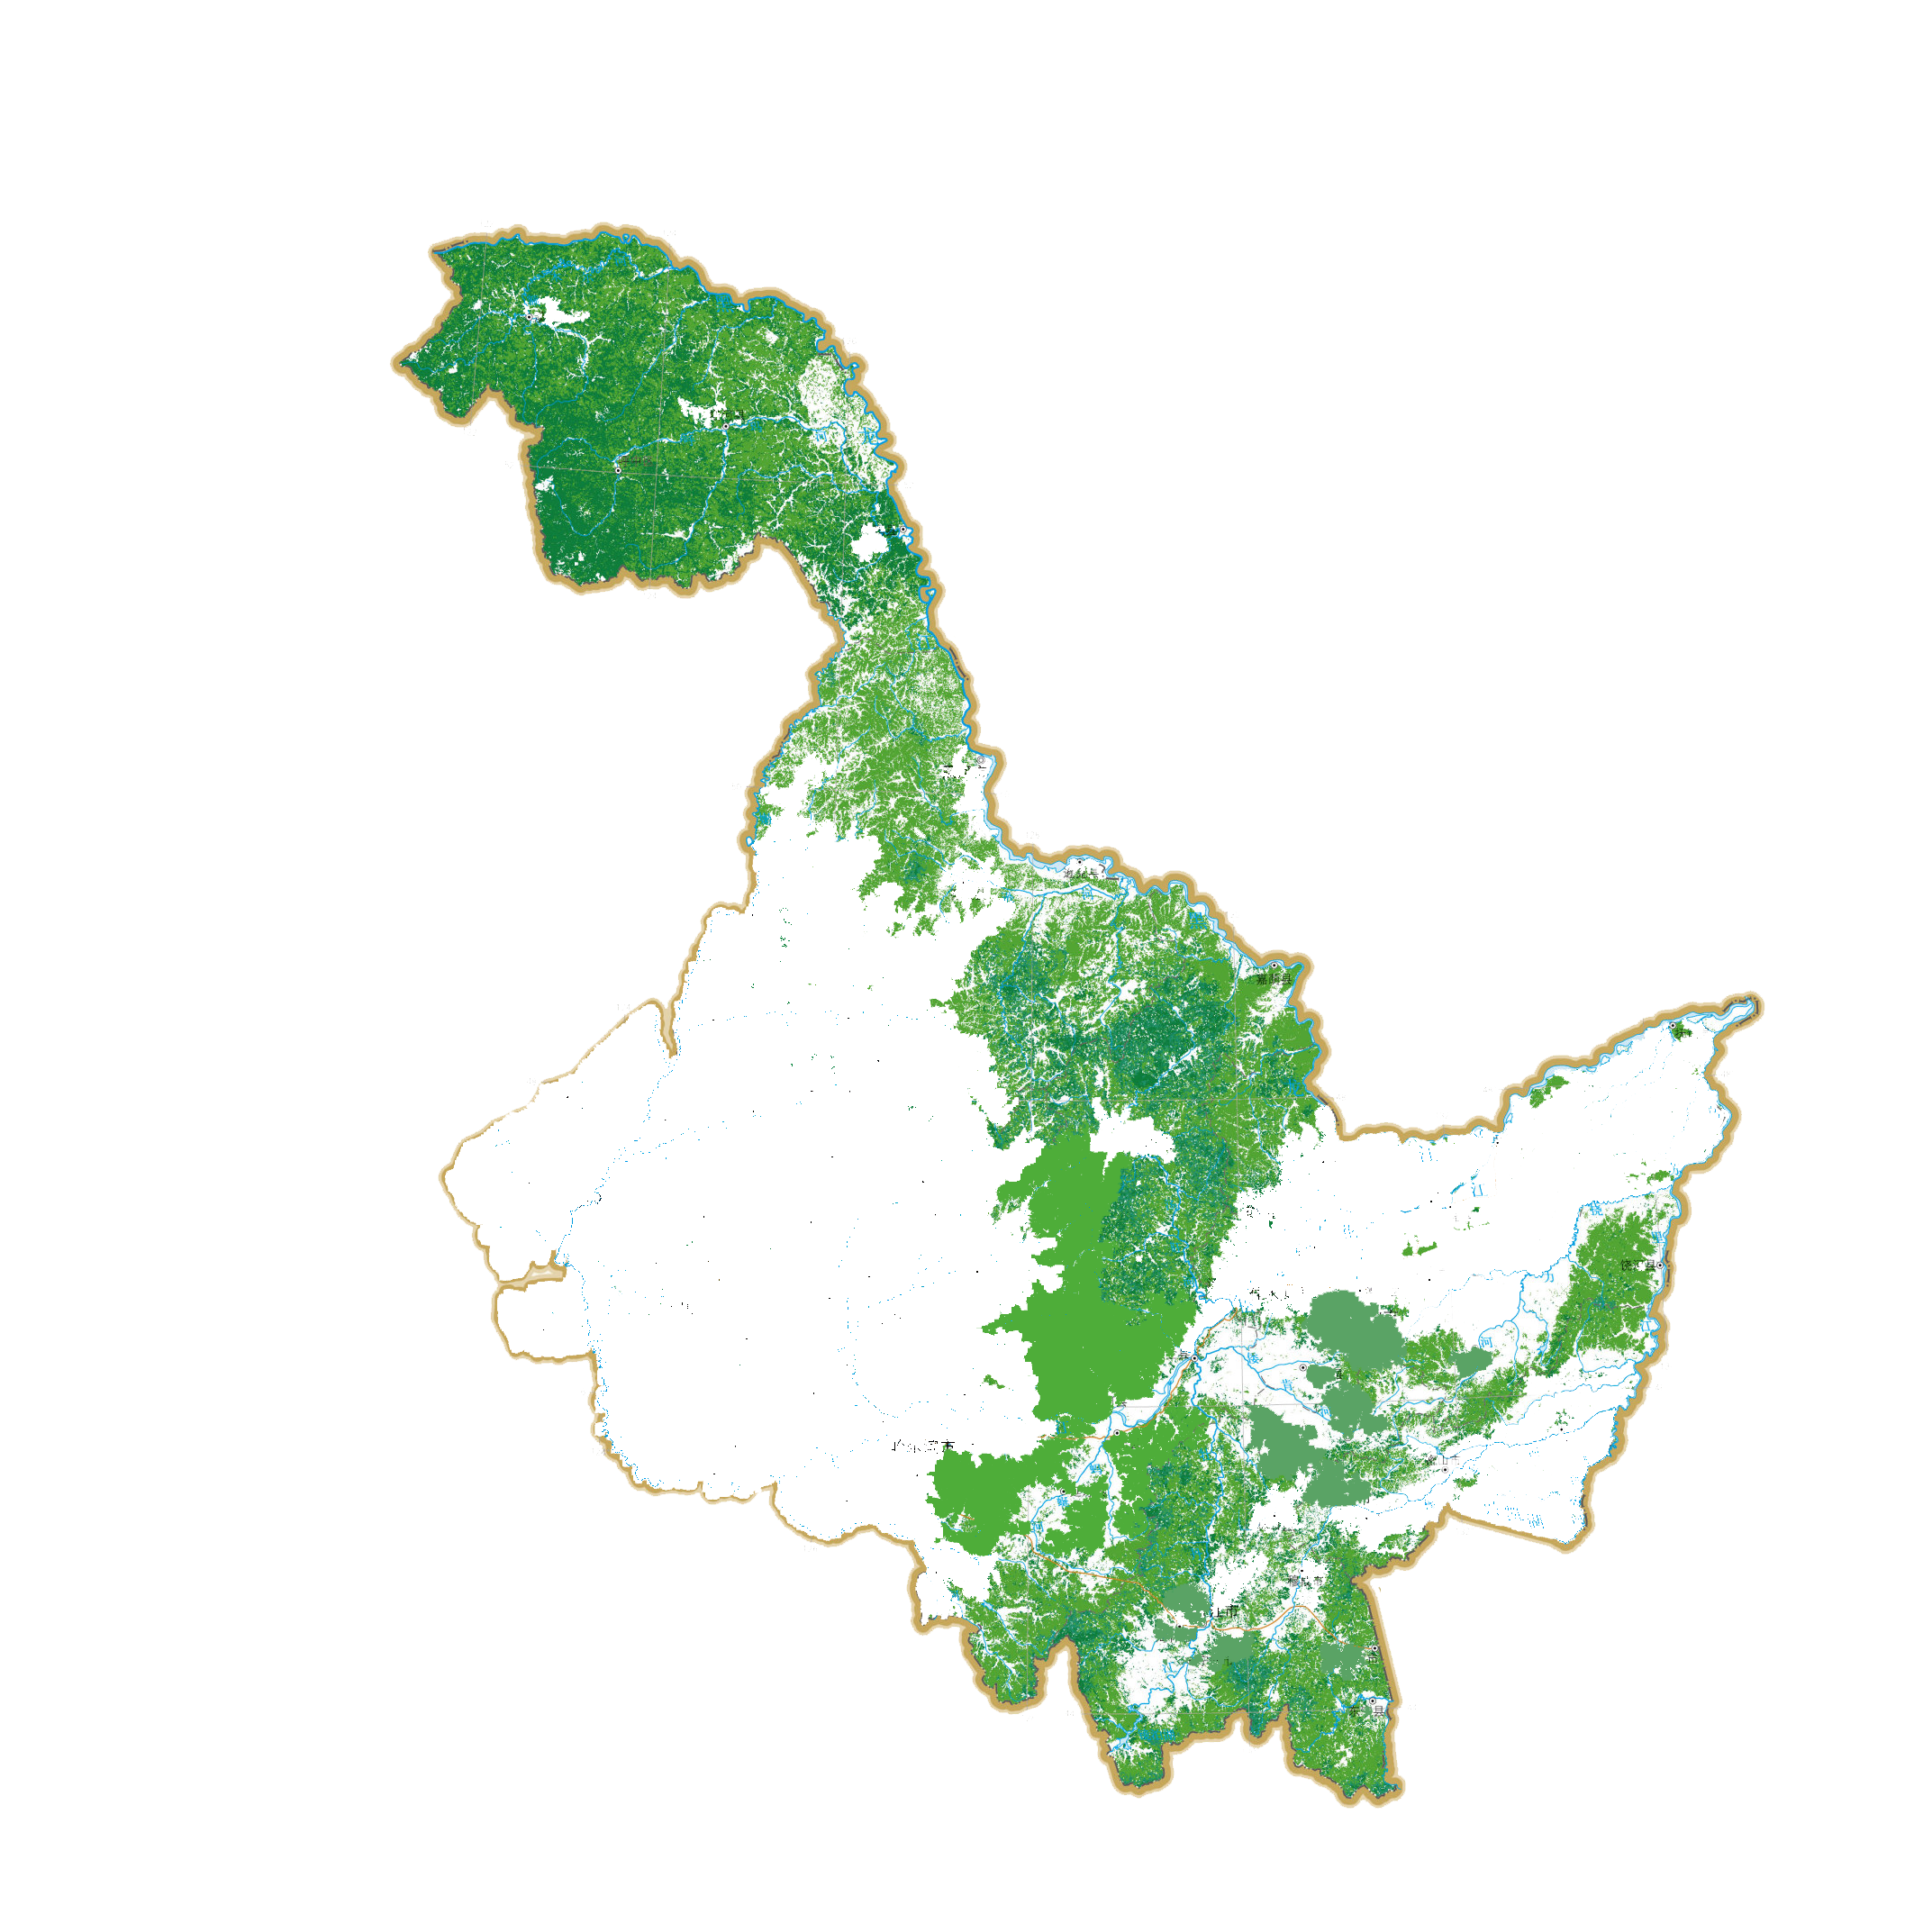
\includegraphics[scale = 0.08]{mcmthesis-demo/figures/heilongjiang.png}
\caption{Forest distribution map of Heilongjiang Province} 
\end{figure}

We log on the official websites of China Meteorological Administration and Forestry Administration to obtain the data required in EEC Value Model from 2010 to 2018, and quantify the forest value of Heilongjiang according to its formula. As shown in the table below.

\begin{table}[h]
	\centering
%   \vspace*{-14cm}              % 调整图像上间距
	\caption{Quantitative forest value in Heilongjiang from 2014 to 2016(billion dollars)}
	\tabulinesep=1mm
	\begin{tabu}to \linewidth{X[0.9,c,m]X[1.4,c,m]X[1.4,c,m]X[1.4,c,m]}
		\tabucline[0.08em]-
		year           & ecologic value    & economic value  &cultural value         \\\tabucline[0.08em]-
		2010      & 55.9578 & 6.9057 & 3.47850 \\
        2011      & 57.2133 & 7.3199 & 3.7113 \\
        2012      & 59.7257 & 7.6231 & 3.9765 \\
        2013      & 61.7045 & 7.8787 & 4.3097 \\
        2014	   & 62.8302      & 8.0561    &4.54694  \\
		2015	   & 67.7652   & 9.6319    &4.5624  \\
		2016	   & 73.0542    &11.1379  &4.5402   \\
        2017       & 74.2948  & 11.5136  &4.9423 \\
        2018      &  75.3012  & 11.6933  &5.2304 \\
        
		\tabucline[0.08em]-
	\end{tabu}
%   \vspace*{-5mm}              % 调整图像下间距
    \label{table5}
\end{table}

\subsubsection{Carbon sequestration stock in the next 100 years}

According to the SHG Simulation Model, we get the maximum annual carbon dioxide storage under the optimal proportion of forest harvest. After accumulation, the total amount of carbon dioxide that can be stored in Heilongjiang forest within 100 years can be obtained. The annual $TCS$ and $\alpha$ is plotted in Fig. [\ref{Forecast line chart}].
\begin{figure}[H]
\centering
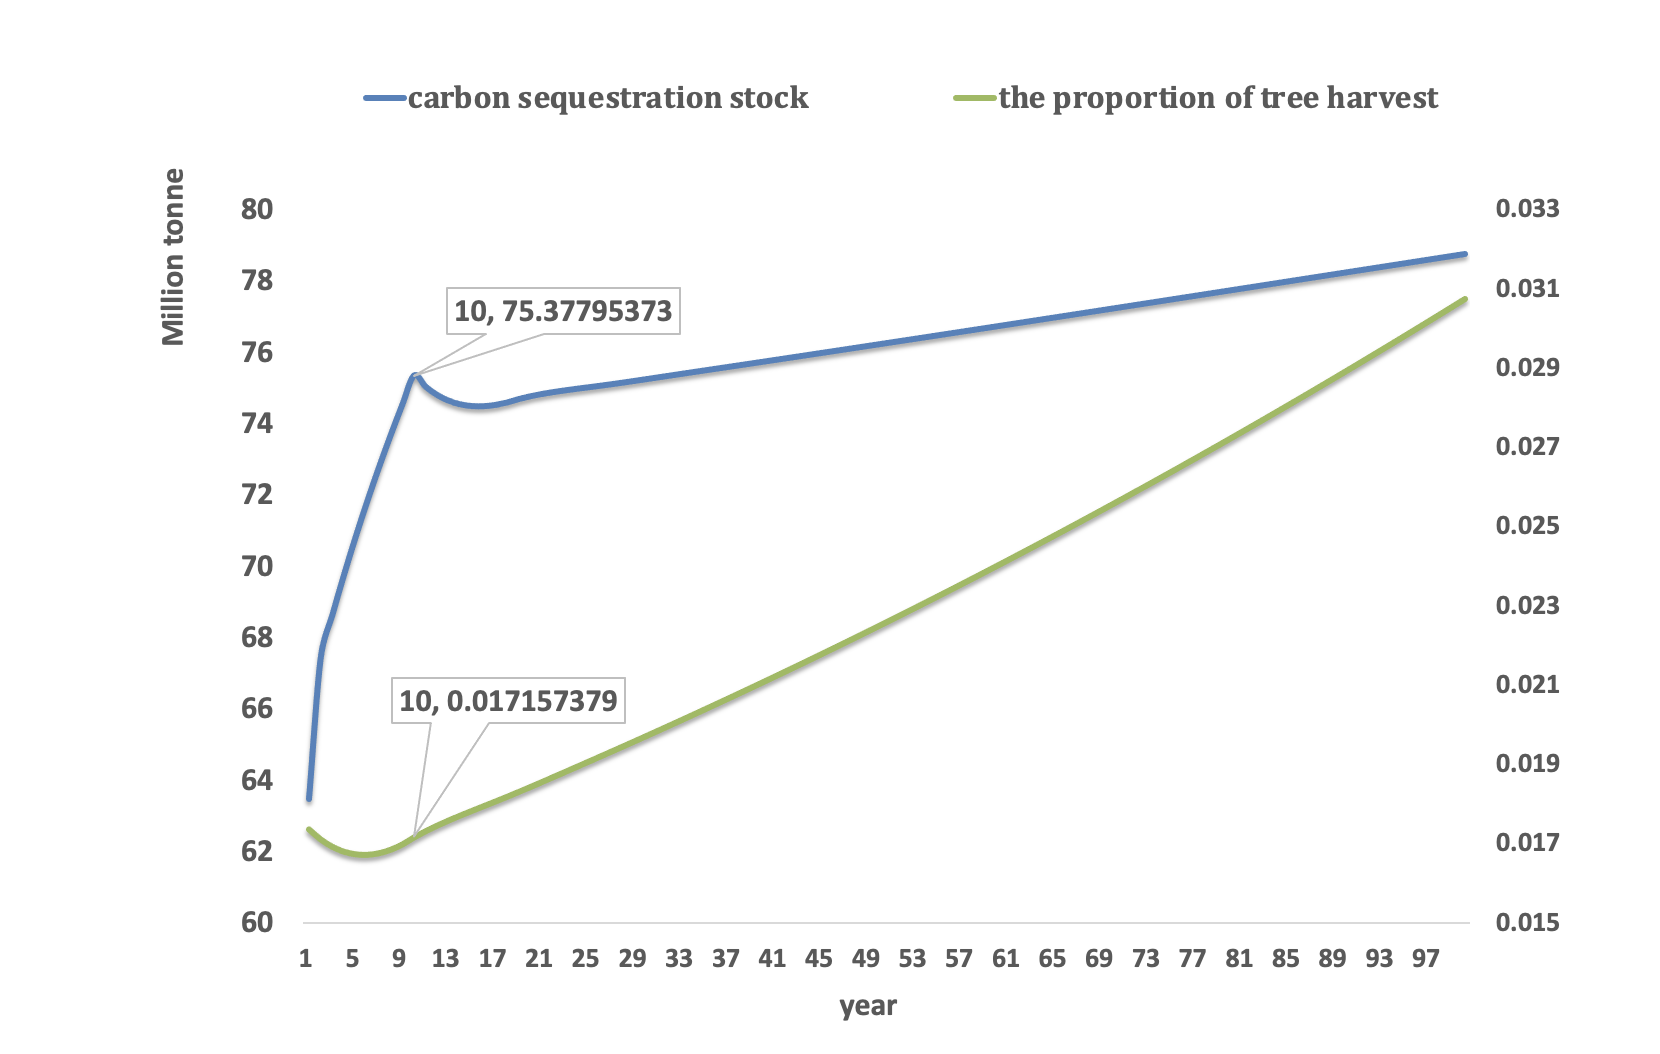
\includegraphics[height = 9cm, width = 14cm]{mcmthesis-demo/figures/Stock.png}
\caption{Forecast line chart of carbon sequestration and proportion of tree harvest}
\label{Forecast line chart}
\end{figure}
According to our model, when the initial $\alpha =0.01767 $ and $\beta = 2.286 $ ,the total amount of the carbon sequestration over 100 years will reach its maximum of $7.599\times 10^9$ tonnes, 15.6 \% more than carbon sequestration taken by untouched forest. So the harvest should be considered in the management plan to maximize the amount of annual carbon sequestration.

\subsubsection{Forest Management Plan in Heilongjiang Forest}

\begin{table}[b]
	\centering
%   \vspace*{-14cm}              % 调整图像上间距
	\caption{the proportion of different forest values in Heilongjiang from 2010 to 2018}
	\tabulinesep=1mm
	\begin{tabu}to \linewidth{X[0.9,c,m]X[1.4,c,m]X[1.4,c,m]X[1.4,c,m]}
		\tabucline[0.08em]-
		year           & ecologic value    & economic value  &cultural value         \\\tabucline[0.08em]-
		2010      &84.34\% & 10.41\% & 5.24\% \\
        2011      & 83.83\% & 10.72\% & 5.43\% \\
        2012      & 83.73\% & 10.68\% & 5.58\% \\
        2013      & 83.50\% & 10.66\% & 5.83\% \\
        2014	   & 83.76\% & 10.67\%   &6.03\% \\
		2015	   & 82.68\%   & 11.75\%   &5.57\% \\
		2016	   & 82.33\%    &12.55\%  &5.11\%   \\
        2017       & 81.87\%  & 12.68\%  &5.45\% \\
        2018      &  81.64\%  & 12.68\%  &5.67\% \\
		\tabucline[0.08em]-
	\end{tabu}
%   \vspace*{-5mm}              % 调整图像下间距
    \label{table6}
\end{table}

Based on the data in Tab. [\ref{table5}], we can calculate the proportion of different forest values in Heilongjiang from 2010 to 2018. We apply the decision tree algorithm to make the analysis about Tab. [\ref{table6}] below, and use the Target Oriented Forest Management Strategy to give proper suggestion on the future direction of forest development.All the conclusions and advice are stated below.



	\begin{itemize}
\item \textbf{Conclusion 1:} Heilongjiang forest has been in the intermediate stage since 2010 according to the decision tree algorithm. The economic value ratio was stable at around 10.5\% and the ecological value ratio was above 80\% for 4 years which indicates that Heilongjiang forest was protected well at that time without deforestation or overuse.
\item \textbf{Conclusion 2:} The transition point during 2010 to 2018 in Heilongjiang forest is 2015 when the economic value ratio was more than 10.8\% and the ecological value ratio was still above 80\%, a symbol of an advanced stage in decision tree algorithm. 
\item \textbf{Suggestion:} Heilongjiang forest can be seen as a stable and advanced forest since 2014 with few possibility that the proportion may change accidently, so the development strategy can be directly into culture-oriented one. Government should explore the underlying value of the forest in cultural layer such education, tourism and scientific research.
	\end{itemize}
    
